\documentclass[thesis.tex]{subfiles}

\begin{document}

\iffulldocument\else
	\chapter{KdV5}
\fi

\section{Generalization of problem}\label{sec:KdV5gen}

\subsection{Hamiltonian PDE}\label{sec:HamPDE}

We will write the problem in general terms, for which KdV5 will be a specific case. This analysis follows \cite{Grillakis1987}. Let $X = H^{2m}(\R)$ and $Y = L^2(\R)$. Consider the PDE
\begin{equation}\label{genPDE}
u_t = \partial_x \calE'(u)
\end{equation}
where $u \in X$ and $\calE(u): X \subset Y \rightarrow \R$ is a smooth functional representing the energy of the system. We take the following hypothesis regarding the energy $\calE(u)$.

\begin{hypothesis}\label{Ehyp}
The energy $\calE(u)$ has the following properties
\begin{enumerate}[(i)]
\item $\calE(0) = 0$ and $\calE'(0) = 0$.
\item $\calE(u)$ is reversible, i.e. $\calE(u) = \calE(\rho(u))$, where $\rho$ is the operator on $X$ defined by $[\rho(u)](x) = u(-x)$.
\item $\calE(u)$ is translation invariant, i.e. $\calE(T(s)u) = \calE(u)$ for all $s \in \R$, where $\{T(s) : s \in \R \}$ is the one parameter group of unitary operators on $X$ defined by $[T(s)]u(\cdot) = u(\cdot - s)$.
\item $\calE'(u): X \rightarrow X$ is a differential operator of the form
\begin{equation}\label{Eprimeuform}
\calE'(u) = \partial_x^{2m}u - f(u, \partial_x u, \dots, \partial_x^{2m-1} u),
\end{equation}
where $f: \R^{2m} \rightarrow \R$ is smooth.
\end{enumerate}
\end{hypothesis}

\noi\cref{Ehyp}(iv) holds in applications such as KdV5, and ensures that we can write the equilibrium equation $\partial_x \calE'(u) = 0$ as a first order system.

Differentiating the reversibility relation $\calE(u) = \calE(\rho(u))$ with respect to $u$, we have
\[
\calE'(u) = \rho^*( \calE'(\rho(u) ) = \rho( \calE'(\rho(u) ),
\]
since $\rho$ is self-adjoint. This implies that the linear part of the operator only involves even-order derivatives of $u$ with respect to $x$. Differentiating the symmetry relation $\calE(T(s)u) = \calE(u)$ with respect to $u$, we have
\begin{equation}\label{Eprimesymm}
\calE'(u) = T(s)^* \calE'(T(s)u) = T(-s) \calE'(T(s)u)
\end{equation}
and
\begin{equation}\label{EHessiansymm}
\calE''(u) = T(s)^* \calE''(T(s)u) T(s).
\end{equation}
Finally, differentating the symmetry relation $\calE(T(s)u) = \calE(u)$ with respect to $s$ at $s = 0$, 
\begin{align*}
0 = \langle \calE'(u), T'(s) u \rangle|_{s = 0}
= \langle \calE'(u), T'(0) u \rangle
= \langle \calE'(u), \partial_x u \rangle
\end{align*}
for all $u \in X$, since $T'(0) = \partial_x$ is the infinitesimal generator of the translation group $T(s)$. The energy $E(u)$ is conserved along solutions $u$ to \cref{genPDE}, since
\[
\frac{d}{dt}\calE(u) = \langle \calE'(u), u_t \rangle = \langle \calE'(u), \partial_x \calE'(u) \rangle = 0,
\]
where we used the fact that the operator $\partial_x$ is skew-symmetric. In addition, there is a second conserved quantity $V: L^2(\R) \rightarrow \R$, given by
\begin{equation}\label{defV}
V(u) = -\frac{1}{2} \int_{-\infty}^\infty u^2 dx,
\end{equation}
which represents charge in some applications. $V(u)$ is also conserved along solutions $u$ to \cref{genPDE}, since
\begin{align*}
\frac{d}{dt}V(u) &= \langle V'(u), u_t \rangle
= \langle -u, \partial_x \calE'(u) \rangle 
= \langle \partial_x u, \calE'(u) \rangle = 0,
\end{align*}
where we used $V'(u) = -u$ in the second equality.

As in \cite{Grillakis1987}, we will study bound states of \cref{genPDE}, which are solutions of the form
\begin{equation}
u(x, t) = T(ct)\phi(x) = \phi(x - ct),
\end{equation}
where $\phi \in X$. Since $T(s)$ is the translation group, these bound states are traveling waves; we will refer to these states as traveling waves from here on. If $\phi$ satisfies the equilibrium equation
\begin{equation}\label{eqODE1}
\calE'(\phi) = c V'(\phi),
\end{equation}
then $T(ct)\phi(x)$ is a traveling wave, since 
\begin{align*}
\frac{d}{dt}T(ct)\phi &= c T'(ct)\phi 
= c T'(0)T(ct)\phi \\
&= \partial_x T(ct) c V'(\phi)
= \partial_x T(ct) \calE'(\phi) \\
&= \partial_x T(ct) T(ct)^* \calE'(T(ct)\phi) \\
&= \partial_x \calE'(T(ct)\phi) 
\end{align*}
Since $V'(\phi) = -\phi$, we can write the equilibrium equation as
\begin{equation}\label{eqODE}
\calE'(\phi) + c \phi = 0.
\end{equation}
Without loss of generality, we will assume that $\calE'(\phi)$ does not contain any terms of the form $b\phi$ for $b$ constant, since those are accounted for by the $c \phi$ term in \cref{eqODE}.

We take the following hypothesis concerning existence of traveling waves. In the next section, we will give a condition under which this hypothesis is satisfied. 
\begin{hypothesis}\label{cintervalhyp}
There exists an open interval $(c_1, c_2) \subset \R$ and a $C^1$ map $c \mapsto \phi_c$ such that for every $c \in (c_1, c_2)$, $\phi_c$ is a traveling wave solution for \cref{genPDE}, i.e. 
\[
\calE'(\phi_c) + c \phi_c = 0.
\]
Furthermore, $\partial_x \phi_c \neq 0$.
\end{hypothesis}

We are interested in the stability of these traveling wave solutions. As a first step in stability analysis, we will look at the spectrum of the linearization of the PDE \cref{genPDE} about a traveling wave. For $c \in (c_1, c_2)$, let $\phi_c$ be a solution to \cref{eqODE}, which is a traveling wave solution to \cref{genPDE}. Then the linearization of the PDE \cref{genPDE} about $\phi_c$ is the linear operator $\partial_x \calL(\phi_c)$ defined by
\begin{equation}\label{PDElinearization}
\partial_x \calL(\phi_c) = 
\partial_x (\calE''(\phi_c) + c )
\end{equation}
where $\calE''(\phi_c)$ is the Hessian of the energy $\calE(\phi_c)$. Both $\calE''(\phi_c)$ and $\calL(\phi_c)$ are self-adjoint. Since $\phi_c$ is a traveling wave, using \cref{Eprimesymm} and \cref{eqODE}, we have
\begin{align}\label{TeqODE}
\calE'(T(s)\phi_c) + c T(s)\phi_c = T(s)[\calE'(\phi_c) + c \phi_c] = 0.
\end{align}
Differentiating \cref{TeqODE} with respect to $s$ at $s = 0$, this becomes
\begin{align*}
0 &= \calE''(T(0)\phi_c)T'(0)\phi_c + c T'(0)\phi_c \\
&= (\calE''(\phi_c) + c ) \partial_x \phi_c \\
&= \calL(\phi_c) \partial_x \phi_c
\end{align*}
Thus $\partial_x \phi_c$ is an eigenfunction of $\calL(\phi_c)$ with eigenvalue 0. Differentiating one more time, $\partial_x \phi_c$ is also an eigenfunction of $\partial_x \calL(\phi_c)$ with eigehvalue 0.

Differentiating \cref{eqODE} with respect to $c$, which we can do because the mapping $c \mapsto \phi_c$ in Hypothesis \ref{cintervalhyp} is $C^1$, we have
\begin{align*}
\calE''(\phi_c)\partial_c \phi_c + c \partial_c \phi_c + \phi_c = 0,
\end{align*}
which we can rearrange to get 
\begin{align*}
(\calE''(\phi_c) + c )(-\partial_c \phi_c) = \phi_c.
\end{align*}
Differentiating both sides, we have
\begin{align*}
\partial_x \calL(\phi_c) (-\partial_c \phi_c) 
= \partial_x (\calE''(\phi_c) + c )(-\partial_c \phi_c) = \partial_x\phi_c.
\end{align*}
Thus $-\partial_c \phi_c$ is a generalized eigenfunction of $\partial_x \calL(\phi_c)$ corresponding to eigenvalue 0.

\subsection{Traveling wave solutons}\label{sec:travelingwaves}

We will look now look at traveling wave solutions to the PDE \cref{genPDE}, which are solutions to equilibrim equation \cref{eqODE}. In particular, we are interested in traveling waves which are exponentially localized. To do this, we will use a spatial dynamics approach. From this viewpoint, an expoentially localized traveling wave is a homoclinic orbit connecting a rest state to itself. To do this, we write \cref{eqODE} as a first order system of ODEs in the standard way. Let $U = (u, \partial_x u, \dots, \partial_x^{2m-1} u)^T \in \R^{2m}$. Then by \cref{Ehyp}(iv), equation \cref{eqODE} is equivalent to the first order system
\begin{equation}\label{genODE}
U'(x) = F(U(x); c),
\end{equation}
where $F: \R^{2m} \times \R \rightarrow \R^{2m}$ is given by
\begin{equation}\label{defF}
F(u_1, u_2, \dots, u_{2m}; c) = 
\begin{pmatrix}
u_2 \\ u_3 \\ \vdots \\ f(u_1, u_2, \dots, u_{2m}) - c u_1
\end{pmatrix}.
\end{equation}
$F$ is smooth, and $F(0; c) = 0$ for all $c$. Reversibility implies that
\begin{equation}\label{genODErev}
F(RU; c) = -RF(U; c),
\end{equation}
where $R:\R^{2m} \rightarrow \R^{2m}$ is the standard reversor operator defined by
\begin{equation}\label{reverserR2m}
R(u_1, u_2, \dots, u_{2m-1}, u_{2m}) = (u_1, -u_2, \dots, u_{2m-1}, -u_{2m}).
\end{equation}
In particular, if $U(x)$ is a solution to \cref{genODE}, so is $RU(-x)$. Taking the derivative of \cref{genODErev} with respect to $U$, it follows that 
\begin{equation}\label{genODErevDF}
D F(RU; c) = -RDF(U; c)R.
\end{equation}
From the last component of \eqref{genODErev}, $f(RU) = f(U)$. It also follows from reversibility that $Df(RU) = RDf(U)$, which implies
\begin{equation}\label{frev}
\begin{aligned}
\partial_{u_j} f(R U) &= (-1)^{j+1} \partial_{u_j} f(U) \\
\partial^2_{u_j u_k} f(R U) &= (-1)^{j+k} \partial^2_{u_j u_k} F(U)
\end{aligned}
\end{equation}
For $U = 0$,
\begin{align}\label{fpartials0}
\partial_{u_j} f(0) &= \begin{cases}
0 & j \text{ even}\\
0 & j = 1 \\
c_j & j \text{ odd, } j > 1
\end{cases}
\end{align}
where the $c_j$ are constants. We can assume without without loss of generality that $c_0 = \partial_{u_1} f(0) = 0$, since that is accounted for by the $c u_1$ term in \cref{defF}.

Next, we assume that \cref{genODE} is a conservative system.

\begin{hypothesis}\label{Hhyp}
There exists a smooth function $H: \R^{2m} \times \R \rightarrow \R$, denoted $H(U; c)$, such that 
\begin{enumerate}[(i)]
\item $H(0; c) = 0$ for all $c$
\item $\nabla_U H(U; c) = 0$ if and only if $F(U; c) = 0$
\item For all $U \in \R^{2m}$ and all $c$,
\begin{equation}
\langle \nabla_U H(U; c), F(U; c) \rangle = 0
\end{equation}
\end{enumerate}
\end{hypothesis}

\noi It follows from \cref{Hhyp} that $H$ is conserved along solutions $U(x)$ to \cref{genODE}. If $U(x)$ is such a solution, then
\[
\frac{d}{dx}H(U(x); c) = \langle \nabla H(U(x); c), U'(x) \rangle
= \langle \nabla H(U(x); c), F(U(x); c) \rangle = 0
\]

Since $F(0; c) = 0$ for all $c$, the rest state $U = 0$ is an equilibrium of \cref{genODE} for all $c$. The next hypothesis addresses the hyperbolicity of this equilibrium. We note that although the eigenvalue pattern described in \cref{hypeqhyp} is not necessary for the existence of a homoclinic orbit, it is a sufficient condition for the existence of multi-pulse solutions.

\begin{hypothesis}\label{hypeqhyp}
For a specific $c_0 \in \R$ with $c_0 > 0$, $U = 0$ is a hyperbolic equilibrium of \cref{genODE}, i.e. $DF(0; c_0)$ has no eigenvalues with real part 0. Furthermore, the spectrum of $DF(0; c_0)$ contains a quartet of simple eigenvalues $\pm \alpha_0 \pm \beta_0 i$, $\alpha_0, \beta_0 > 0$, and for any other eigenvalue $\nu$ of $DF(0; c_0)$, $|\text{Re }\nu| > \alpha_0$.
\end{hypothesis}

Let $W^s(0; c_0)$ and $W^u(0; c_0)$ be the stable and unstable manifolds of the equilibrium at 0, and let $E_0^s(c_0)$ and $E_0^u(c_0)$ be the stable and unstable eigenspaces of $DF(0; c_0)$. By reversibility, these spaces have dimension $m$. The stable and unstable manifolds are smooth since $F$ is smooth.

\subsection{Primary pulse solution}\label{sec:primarypulse}

We now address the existence of a primary pulse solution, which is a symmetric homoclinic orbit connecting the rest state equilibrium to itself. In general, the existence of such a solution is unknown, although in specific cases such as KdV5 we do have an existence result. Thus we will take the existence of a primary pulse solution as a hypothesis.

\begin{hypothesis}\label{Qexistshyp}
For the same $c_0$ as in \cref{hypeqhyp}, there exists a homoclinic orbit solution $Q(x; c_0) \in W^s(0) \cap W^u(0) \subset H^{-1}(0)$ to \cref{genODE}. In addition,
\begin{enumerate}[(i)]
\item $Q(0; c_0) \neq 0$
\item $\nabla_U H(Q(0; c_0); c_0) \neq 0$
% \item $\partial_c H(Q(0; c_0); c_0) \neq 0$
\item $Q(x; c_0)$ is symmetric with respect to the reversor operator \cref{reverserR2m}, i.e. $Q(-x; c_0) = R Q(x; c_0)$
\end{enumerate}
\end{hypothesis}

\noi Since we obtained \cref{genODE} by putting \cref{eqODE} into a first order system in the standard way, 
\begin{equation}\label{Qqrelation}
Q(x; c_0) = (q(x; c_0), \partial_x q(x; c_0), \dots, \partial_x^{2m-1}q(x; c_0))^T,
\end{equation}
where $q(x; c_0)$ is an even function and is an exponentially localized traveling wave solution solution to \cref{genPDE}. 

Next, we address the intersection of the stable and unstable manifolds $W^s(0; c_0)$ and $W^u(0; c_0)$. By \cref{Hhyp}, $W^s(0; c_0), W^u(0; c_0) \subset H^{-1}(0; c_0)$, where $H^{-1}(0; c_0)$ is the 0-level set of $H$. We have the following lemma concerning $H^{-1}(0; c_0)$.

\begin{lemma}\label{manifoldinH0}
There exists $\delta > 0$ such that for $c \in (c_0 - \delta, c_0 + \delta)$, the zero level set $H^{-1}(0; c)$ contains a smooth $(2m-1)$-dimensional manifold $M(c)$; $M(c_0)$ contains $Q(0; c_0)$.
\end{lemma}

We then take the following hypothesis regarding the intersection of the stable and unstable manifolds in $H^{-1}(0; c_0)$.

\begin{hypothesis}\label{H0transversehyp}
The stable manifold $W^s(0; c_0)$ and the unstable manifold $W^u(0; c_0)$ intersect transversely in $H^{-1}(0; c_0)$ at $Q(0; c_0)$.
\end{hypothesis}

\noi By \cref{H0transversehyp} and \cref{manifoldinH0}, 
\[
\dim (T_{Q(0; c_0)}W^s(0; c_0) + T_{Q(0; c_0)}W^u(0; c_0)) = \dim M(c_0) = 2m-1 
\]
Since $\dim T_{Q(0; c_0)}W^s(0; c_0) = m$ and $\dim T_{Q(0; c_0)}W^s(0; c_0) = m$, by a dimension-counting argument, $\dim T_{Q(0; c_0)}W^s(0; c_0) \cap T_{Q(0; c_0)}W^u(0; c_0) = 1$. Since $Q(x; c_0) \subset W^s(0; c_0) \cap W^u(0; c_0)$, 
\[
Q'(0; c_0) \in T_{Q(0; c_0)}W^s(0; c_0) \cap T_{Q(0; c_0)}W^u(0; c_0),
\]
thus we have the nondegeneracy condition
\begin{equation}\label{nondegencond}
T_{Q(0; c_0)}W^s(0; c_0) \cap T_{Q(0; c_0)}W^u(0; c_0) = \R Q'(0; c_0)
\end{equation}
 
Using \cref{nondegencond}, we can decompose the tangent spaces of the stable and unstable manifolds at $Q(0; c_0)$. Since the two tangent spaces have a one-dimensional intersection spanned by $Q'(0; c_0)$, we can decompose them as 
\begin{equation}\label{TQ0decomp1}
\begin{aligned}
T_{Q(0; c_0)}W^u(0; c_0) &= \R Q'(0; c_0) \oplus Y^-(c_0) \\
T_{Q(0; c_0)}W^s(0; c_0) &= \R Q'(0; c_0) \oplus Y^+(c_0)
\end{aligned}
\end{equation}

We can now prove the existence of homoclinic orbits $Q(x; c)$ for $c$ near $c_0$ and show that $Q(x; c)$ is differentiable in $c$.

\begin{theorem}\label{transverseint}
Assume \cref{Hhyp} and \cref{H0transversehyp}. Then there exists $\delta > 0$ with the following property. For $c \in (c_0 - \delta, c_0 + \delta)$, the stable and unstable manifolds $W^s(0; c)$ and $W^u(0; c)$ have a one-dimensional transverse intersection in $H^{-1}(0; c)$. This intersection yields a homoclinic orbit $Q(x; c)$. The map $c \rightarrow Q(x; c)$ is smooth, and the derivative $\partial_c Q(x; c)$ is exponentially localized. Specifially, for any $\epsilon > 0$, there exists $\delta_1 > 0$ with $\delta_1 < \delta$ such that for $c \in (c_0 - \delta_1, c_0 + \delta_1)$,
\[
|\partial_c Q(x; c)| \leq C e^{-(\alpha - \epsilon)|x|}
\] 
\end{theorem}
 
\noi \cref{transverseint} implies that \cref{cintervalhyp} is satisfied. From this point forward, we will fix $c = c_0$, and for simplicity, we will use $c$ in place of $c_0$. We will also omit the dependence on $c$ for convenience of notation.

\subsection{Variational equation}\label{sec:vareq1}

The variational equation is the linearization of \cref{genODE} about the primary pulse solution $Q(x)$. The variational and adjoint variational equations associated with \cref{genODE} are
\begin{align}
V' = DF(Q(x)) V \label{vareq1} \\
W' = -DF(Q(x))^* W \label{adjvareq1},
\end{align}
where $DF(Q(x))$ is the $2m \times 2m$ matrix
\begin{equation}\label{defDF}
DF(Q(x)) = 
\begin{pmatrix}
0 & 1 & 0 & \dots & 0 & 0 \\
0 & 0 & 1 & \dots & 0 & 0 \\
& && \ddots \\
0 & 0 & 0 & \dots & 1 & 0 \\
0 & 0 & 0 & \dots & 0 & 1 \\
\partial_{u_1}f(Q(x)) - c & \partial_{u_2}f(Q(x)) & \partial_{u_3}f(Q(x)) & \dots & \partial_{u_{2m-1}}f(Q(x)) & \partial_{u_{2m}}f(Q(x))
\end{pmatrix}
\end{equation}
It follows from \cref{nondegencond} that $Q'(x)$ is the unique bounded solution to \cref{vareq1}, and that there exists a unique bounded solution $\Psi(x)$ to \cref{adjvareq1}. (In both cases, uniqueness is up to scalar multiples). Since we have a conserved quantity $H$, we know the exact form of $\Psi(x)$, which is given in the following lemma.

\begin{lemma}\label{psiform}
The unique bounded solution $\Psi(x)$ to the adjoint variational equation \cref{adjvareq1} is given by $\Psi(x) = \nabla H(Q(x))$. In addition, $\Psi(x)$ is symmetric with respect to the standard reversor operator $R$, i.e. $\Psi(-x) = R \Psi(x)$, and
the last component of $\Psi(x)$ is $q'(x)$.
\end{lemma}

The last lemma of the section collects a few important results about solutions to the variational and adjoint variational equations.

\begin{lemma}\label{eigadjoint}
Consider the linear ODE $V' = A(x)V$ and the corresponding adjoint equation $W' = -A(x)^* W$, where $A$ is an $n \times n$ matrix depending on $x$. Then the following are true.
\begin{enumerate}[(i)]
\item $\dfrac{d}{dx}\langle V(x), W(x) \rangle = 0$, thus the inner product is constant in $x$.
\item If $W(x)$ is bounded and $V(x) \rightarrow 0$ as $x \rightarrow \infty$ or $V(x) \rightarrow -\infty$, then $\langle V(x), W(x) \rangle = 0$ for all $x \in \R$. The same holds if we reverse the roles of $W$ and $V$.
\item If $\Phi(y, x)$ is the evolution operator for $V'(x) = A(x)V(x)$, then $\Phi(x, y)^*$ is the evolution operator for the adjoint equation $W'(y) = -A(y)^* W(y)$.
\end{enumerate}
\end{lemma}

\noi From \cref{eigadjoint}(ii), $\Psi(0) \perp \R Q'(0) \oplus Y^+ \oplus Y^-$, thus we can decompose $\R^{2m}$ as
\begin{equation}\label{R2mdecomp}
\R^{2m} = \R Q'(0) \oplus Y^+ \oplus Y^- \oplus \R \Psi(0).
\end{equation}

\subsection{PDE eigenvalue problem}\label{sec:PDEeig}

Let $\phi$ be a traveling wave solution to \cref{genPDE}, i.e. $\phi$ satisfies \cref{eqODE}. To study the spectral stability of $\phi$, we will look at the PDE eigenvalue problem
\begin{equation}\label{genPDEeig}
\partial_x \calL_c v = \lambda v
\end{equation}
where $\calL_c$ is defined in equation \cref{PDElinearization}. As in \cref{sec:travelingwaves}, we will take a spatial dynamics approach and write \cref{genPDEeig} as a first order system of ODEs. First, we write \cref{genPDEeig} as the system
\[
\begin{aligned}
\calL_c v &= k \\
\partial_x k &= \lambda v
\end{aligned}
\]
From \cref{Eprimeuform} and \cref{PDElinearization}, 
\[
\calL_c = \partial_x^{2m}u - f(u, \partial_x u, \dots, \partial_x^{2m-1} u) + c
\]
where $f: \R^{2m} \rightarrow \R$ is smooth. Let $V = (v, \partial_x v, \dots, \partial_x^{2m-1} v, k) \in \R^{2m+1}$. Then \cref{genPDEeig} is equivalent to the first order system
\begin{equation}\label{PDEeigsystem}
V'(x) = A(\phi(x))V(x) + \lambda B V(x)
\end{equation}
where $A(\phi(x))$ is the $(2m+1)\times(2m+1)$ matrix
\begin{equation}\label{defAphi}
A(\phi(x)) = 
\begin{pmatrix}
0 & 1 & 0 & \dots & 0 & 0 & 0 \\
0 & 0 & 1 & \dots & 0 & 0 & 0\\
& \vdots && \vdots \\
0 & 0 & 0 & \dots & 0 & 1 & 0 \\
f_{u_1}(\phi) - c & f_{u_2}(\phi) & f_{u_3}(\phi) & \dots & f_{u_{2m-1}}(\phi) & f_{u_{2m}}(\phi) & 1 \\
0 & 0 & 0 & \dots & 0 & 0 & 0
\end{pmatrix}
\end{equation}
and $B$ is the $(2m+1) \times (2m+1)$ constant coefficient matrix
\begin{equation}\label{DefB}
B = \begin{pmatrix}0 & 0 & 0 & 0 & 0 \\0 & 0 & 0 & 0 & 0 \\  & 
\vdots & & \vdots & \\0 & 0 & 0 & 0 & 0 \\1 & 0 & 0 & 0 & 0 \end{pmatrix} 
\end{equation}
We note that the upper left $2m \times 2m$ block of $A(\phi(x))$ is $DF(\phi(x))$.

Since $\phi$ is a traveling wave, it is exponentially localized, thus $A(\phi(x))$ is exponentially asymptotic to the constant coeffient matrix $A(0)$. The following lemma describes the eigenvalues and kernel of $A(0)$.

\begin{lemma}\label{eigA0lemma}
The following hold concerning the eigenvalues of $A(0)$.
\begin{enumerate}[(i)]
\item $A(0)$ has a simple eigenvalue at 0 and a quartet of eigenvalues at $\pm \alpha_0 \pm \beta_0 i$. For any other eigenvalue $\nu$ of $A(0)$, $|\text{Re }\nu| > \alpha_0$.
\item The kernel of $A(0)$ is spanned by $V_0$ and the kernel of $A^*(0)$ is spanned by $W_0$, where
\begin{align}
V_0 &= (1/c, 0, \dots, 0, 1)^T \label{V0} \\
W_0 &= (0, 0, \dots, 0, 1)^T \label{W0}
\end{align}
We note that $\langle V_0, W_0 \rangle = 1$.
\item The projection on the kernel of $A(0)$ is given by
\begin{equation}\label{projkernelA0}
P_{\ker A(0)} = \langle W_0, \cdot \rangle V_0
\end{equation}
\end{enumerate} 
\end{lemma}

Since $A(0)$ is not hyperbolic, the results of \cite{Sandstede1998} do not apply. Let $W^s(0)$, $W^u(0)$, and $W^c(0)$ be the stable, unstable, and center manifolds of the equilibrium at 0. (These are not the same as in the previous section, but we will retain the notation for convenience). By reversibility, $\dim W^s(0) = m$ and $\dim W^u(0) = m$. The center manifold $W^c(0)$ is one-dimensional.

The variational and adjoint variational equations associated with \cref{PDEeigsystem} are
\begin{align}
V'(x) = A(Q(x)) V(x) \label{vareq2} \\
W'(x) = -A(Q(x))^* W(x) \label{adjvareq2}
\end{align}
We note that these are different than the variational and adjoint variational equations in \cref{sec:vareq1}, but we retain the same notation for convenience. Let 
\[
Q(x) = (q(x), \partial_x q(x), \dots, \partial_x^{2m-1} q(x), 0)\]
be the primary pulse solution from \cref{sec:primarypulse} with an additional component of 0 added to the end since we are now in $\R^{2m+1}$. Again, we keep the same notation for the primary pulse for convenience. 

Since $(\partial_x \calL_c)(\partial_x q) = 0$, it follows that $Q'(x)$ is an exponentially localized solution to the variational equation \eqref{vareq2}, i.e. 
\begin{equation}\label{Qprimevarsol}
(\partial_x Q(x))' = A(Q(x))(\partial_x Q(x))
\end{equation}
Since $(\calL_c \partial_x)(-\partial_c q) = \partial_x q$, we also have
\begin{equation}\label{Qcvarsol}
(\partial_c Q(x))' = A(Q(x))(\partial_c Q(x)) + B(\partial_x Q(x))
\end{equation}

Since $Q(x)$ is exponentially localized, it cannot involve the center manifold $W^c(0)$, thus it must lie in the intersection of the stable and unstable manifolds. In particular, this implies that $\R Q'(0) \subset T_{Q(0)}W^s(0) \cap T_{Q(0)}W^u(0)$. It follows from \cref{H0transversehyp} that these are actually equal, which we state in the following lemma.

\begin{lemma}\label{nondegenlemma}
We have the nondegeneracy condition
\begin{equation}\label{nondegen2}
T_{Q(0)}W^s(0) \cap T_{Q(0)}W^u(0) = \R Q'(0)
\end{equation}
\end{lemma}

Using the nondegeneracy condition \eqref{nondegen2}, we can decompose the tangent spaces of the stable and unstable manifolds at $Q(0)$ as
\begin{align*}
T_{Q(0)}W^s(0) &= \R Q'(0) \oplus Y^+ \\
T_{Q(0)}W^u(0) &= \R Q'(0) \oplus Y^- \\
\end{align*}
Since $\dim \R Q'(0) \oplus Y^+ \oplus Y^- = 2m-1$, there are two remaining directions needed in order to span $\R^{2m+1}$. To find these, we will use the following two lemmas regarding solutions to \eqref{vareq2} and \eqref{adjvareq2}.

\begin{lemma}\label{varadjsolutions}
We have the following solutions to the variational equation and adjoint variational equation.
\begin{enumerate}
	\item There exists a bounded solution $V^c(x)$ to \eqref{vareq2} such that 
	\begin{equation}
	V^c(x) \rightarrow V_0 \text{ as }|x| \rightarrow \infty
	\end{equation}
	$V^c$ is symmetric with respect to the standard reversor operator $R$, i.e. $V^c(-x) = R V^c(x)$.

	\item There exist two linearly independent, bounded solutions $\Psi(x)$ and $\Psi^c(x)$ to \eqref{adjvareq2}.
	\begin{enumerate}[(i)]
	\item $\Psi(x)$ is the exponentially localized solution
	\begin{equation}
	\Psi(x) = (\nabla H(Q(x)), q(x)).
	\end{equation}
	$\Psi(x)$ is symmetric with respect to the standard reversor operator $R$, i.e. $\Psi(-x) = R \Psi(x)$. 
	\item $\Psi_c(x)$ is the constant solution
	\begin{equation}
	\Psi^c(x) = W_0
	\end{equation}
	\end{enumerate}
	Any other bounded solution to \eqref{adjvareq2} is a linear combination of these. Finally, $\Psi(0), \Psi^c(0) \perp \R Q'(0) \oplus Y^+ \oplus Y^-$.
\end{enumerate}
\end{lemma}

Using Lemma \ref{nondegenlemma} and Lemma \ref{varadjsolutions}, we can decompose $\R^{2m+1}$ as  
\begin{equation}
\R^{2m+1} = \R \Psi(0) \oplus \R \Psi^c(0) \oplus \R Q'(0) \oplus Y^+ \oplus Y^-
\end{equation}
where $\R \Psi(0) \oplus \R \Psi^c(0) \perp \R Q'(0) \oplus Y^+ \oplus Y^-$.

The final hypothesis concerns a higher order Melnikov integral. Before we consider that, we note that the standard Melnikov integral is 0, i.e. 
\begin{equation}\label{M1}
M_1 = \int_{-\infty}^\infty \langle \Psi(x), B Q'(x) \rangle =
\int_{-\infty}^\infty q(x) \: \partial_x q(x) 
= \langle q(x), \partial_x q(x) \rangle_{L^2(\R)} = 0
\end{equation}
since the last component of $\Psi(x)$ is $q(x)$ by Lemma \ref{varadjsolutions}, and $q(x)$ is an even function. We take the following hypothesis regarding a higher order Melnikov integral.
\begin{hypothesis}\label{Melnikov2hyp}
The following higher order Melnikov integral is nonzero.
\begin{equation}\label{M2}
M_2 = \int_{-\infty}^\infty \langle \Psi(x), B Q_c(x) \rangle dx =
\int_{-\infty}^\infty q(x) q_c(x) dx \neq 0
\end{equation}
\end{hypothesis}
In applications such as KdV5, numerical analysis suggests that \cref{Melnikov2hyp} is satisfied with $M_2 > 0$.

\section{Multi-pulses on the real line}\label{sec:multiR}

\subsection{Existence}\label{sec:multiexistR}

A multi-pulse is a localized, multi-modal solution $q_n(x)$ to \cref{eqODE} which resembles $n$ well-separated copies of the primary pulse $q(x)$. From a spatial dynamics perspective, a multi-pulse is a multi-loop homoclinic orbit solution $Q_n(x)$ to \eqref{genODE} which stays close to the primary pulse solution $Q(x)$. $Q_n(x)$ and $q_n(x)$ are related as in \cref{Qqrelation}. Heuristically, we construct a multi-pulse by glueing together multiple copies of the primary pulse end-to-end. This is shown in \cref{fig:multipulsediag}.

\begin{figure}[H]
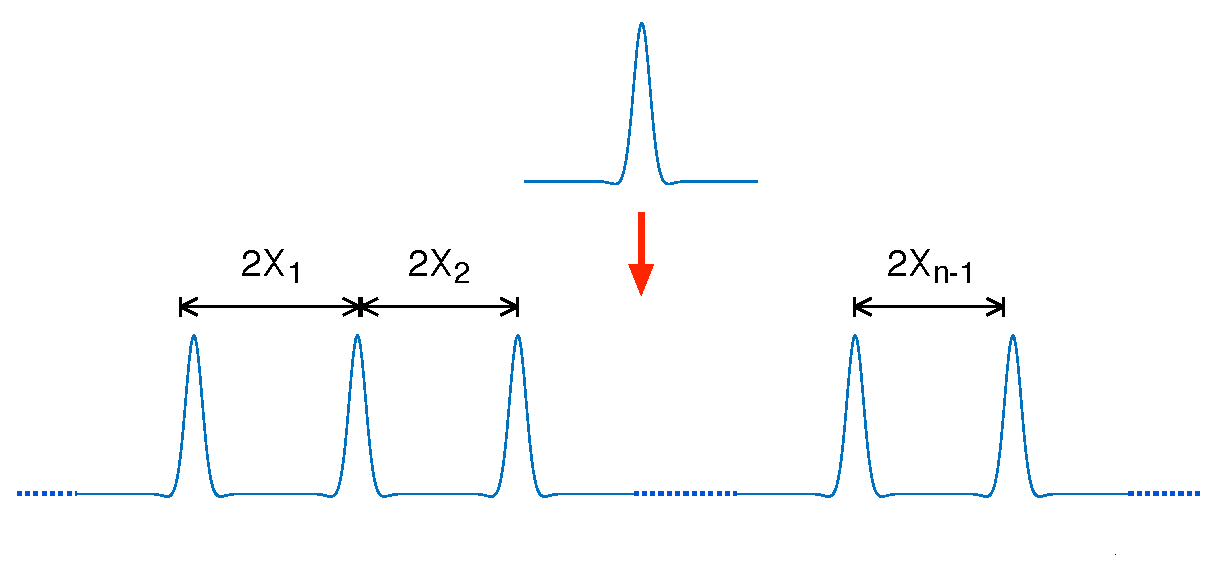
\includegraphics[width=12cm]{images/kdv5numerics/multipulse.eps}
\caption{Construction of a multi-pulse solution from the primary pulse.}
\label{fig:multipulsediag}
\end{figure}

An $n$-pulse $q_n$ can be characterized by $n-1$ pulse distances $\{ X_1, \dots, X_{n-1} \}$; the distance between consecutive peaks is $2 X_j$. Rather than using describing a multi-pulse by the pulse distances, we will use the parameterization from \cite{SandstedeStrut}, which has a built-in scaling parameter and is much simpler to work with mathematially. An $n-$pulse is described using the following parameters:
\begin{enumerate}
\item A scaling parameter $r \in \calR$ with $r > 0$, where
\[
\calR = \left\{ \exp\left(-\frac{2 \pi \alpha_0}{\beta_0}m \right) : m \in \N_0 \right\}
\]
\item A sequence of $n-1$ baseline length parameters $\{ b_1^0, \dots, b_{n-1}^0 \}$, where 
\[
b_j = \exp\left(-\frac{\pi \alpha_0}{\beta_0}m_j \right)
\]
for $m_j \in \N_0$, and we have the additional restriction that $m_j \in \{0, 1\}$ for some $j$.
\end{enumerate}

The following theorem, which is adapted from \cite[Theorem 3.6]{SandstedeStrut} states the existence result for multi-pulse solutions.

\begin{theorem}[Existence of Multi-Pulses]\label{multipulseexistR}
Assume Hypotheses \ref{Ehyp}, \ref{Hhyp}, \ref{hypeqhyp}, \ref{Qexistshyp}, and \ref{H0transversehyp}. There exists $\delta > 0$ such that for any $n \geq 2$ the following holds. For any sequence of baseline length parameters $\{ b_1^0, \dots, b_{n-1}^0 \}$, there exists $r_0 \in \calR$, $r_0 > 0$ with the following property.
\begin{enumerate}[(i)]
\item For every scaling parameter $r \in \exp\left(-\frac{2 \pi \alpha_0}{\beta_0}m \right) \in \calR$ with $0 < r \leq r_0$ there exists a unique $n$-pulse solution $Q_n$ to \cref{genODE} which resembles $n$ consecutive copies of $Q$. The distances between consecutive peaks are given by
\[
2 X_j = \frac{\pi}{\beta_0}(2 m + m_j) + R_j(r) + \tilde{L}
\]
where $\tilde{L}$ is a constant and the remainder terms $R_j(r) \rightarrow 0$ as $r \rightarrow 0$.

\item There are exactly $n$ real eigenvalues $\lambda_j$ of $\calE''(q_n)$ with $|\lambda_j| < \delta$. These are as follows.
\begin{enumerate}
	\item There are $n_{\text{odd}}$ negative eigenvalues, where $n_{\text{odd}}$ is the number of $m_j$ which are odd.
	\item There are $n_{\text{even}}$ positive eigenvalues, where $n_{\text{even}}$ is the number of $m_j$ which are even.
	\item There is a simple eigenvalue at 0 with corresponding eigenfunction $\partial_x Q_n$.
\end{enumerate}

\item We can write $Q_n(x)$ as a piecewise perturbation of the primary pulse $Q(x)$ composed of the $2n$ pieces $\{ Q_j^\pm(x) : j = 1, \dots, n \}$, where $Q_j^-: [-X_{j-1}, 0] \rightarrow \R^{2m}$ and $Q_j^+: [0, X_j] \rightarrow \R^{2m}$, with $X_0 = X_n = \infty$. The pieces are joined together end-to-end as in \cite{Sandstede1998}. We can write the $Q_j^\pm(x)$ as 
\begin{equation}\label{Qpmexpansions}
Q_j^\pm(x) = Q(x) + \tilde{Q}_j^\pm(x)
\end{equation}
where $\tilde{Q}_j^\pm(x)$ are small remainder terms, and we have the estimates
\begin{equation}
\begin{aligned}
\|\tilde{Q}_j^\pm\| &\leq C e^{-\alpha_0 X_m} \\
|\tilde{Q}_{j+1}^-(-X_j) - Q(X_j)| &\leq C e^{-2 \alpha_0 X_m} \\
|\tilde{Q}_j^+(X_j) - Q(-X_j)| &\leq C e^{-2 \alpha_0 X_m} \\
\end{aligned}
\end{equation}
which hold in addition for derivatives of $Q$.
\end{enumerate}
\begin{proof}
Parts (i) and (ii) follow from \cite{SandstedeStrut}. We will show that the hypotheses in \cite{SandstedeStrut} are satisfied. \cref{hypeqhyp} and \cref{Hhyp} are equivalent to Hypotheses 3.1 and 3.3 in \cite{SandstedeStrut}. The eigenvalue problem corresponding to \cref{genODE} is
\[
V'(x) = (\calE''(q_n(x)) + \lambda B )V(x)
\]
where $B$ is a $2m\times 2m$ matrix of the same form as \cref{DefB}. The relevant Melnikov integral is
\[
M = \int_{-\infty}^\infty \langle \Psi(x), B \frac{d}{dx} Q(x) \rangle  dx = \int_{-\infty}^\infty q'(x)^2 dx > 0
\]
since the last component of $\Psi_(x)$ is $q'(x)$ by \cref{psiform}. Thus Hypotheses 3.5 in \cite{SandstedeStrut} is satisfied. The result follows from \cite[Theorem 3.6]{SandstedeStrut}. Since $\calE''(q_n)$ is self-adjoint, its eigenvalues are real.

Part (iii) follows from \cite[Theorem 2]{Sandstede1998}, which follow from \cite{Sandstede1993}.
\end{proof}
\end{theorem}

\subsection{Eigenvalue problem}\label{sec:multispecR}

Let $Q_n(x)$ be a multi-pulse solution to \cref{genODE} constructed using \cref{multipulseexistR}, and let $q_n(x)$ be the first component of $Q_n(x)$; $q_n(x)$ is a traveling wave solution to \eqref{genPDE}. To find the spectrum associated with $q_n$, we study the PDE eigenvalue problem \cref{genPDEeig}. 

First, we look at the essential spectrum. Since any traveling wave solution we are considering is exponentially asymptotic to the rest state $u = 0$, by the Weyl essential spectrum theorem \cite[Theorem 2.2.6]{Kapitula2013} and \cite[Theorem 3.1.11]{Kapitula2013}, $\partial_x \calL_c''(q_n)$ and $\partial_x \calL_c''(0)$ have the same essential spectrum. Using \cref{fpartials0}, the eigenvalue problem for $u = 0$ is 
\[
(\partial_x \calL_c''(0) - \lambda )v(x) = 
(\partial_x^{2m+1} + c_{2m-1} \partial_x^{2m-1} + \dots + c_3 \partial_x^3 + c \partial_x - \lambda )v(x) = 0
\]
Using \cite[(3.1.20)]{Kapitula2013}, the essential spectrum is given by the curve
\begin{align}\label{essspecR}
\lambda(k) &= \{ (ik)^{2m+1} + c_{2m-1} (ik)^{2m-1} + \dots + c_3 (ik)^3 + c (ik) : k \in \R \}
\end{align}
which is purely imaginary since all powers of $i$ are odd. Thus the essential spectrum is a subset of the imaginary axis. Furthermore, replacing $k$ with $-k$ in \cref{essspecR}, the essential spectrum is symmetric about the real axis. In many cases, such as KdV5, the essential spectrum is the entire imaginary axis, although that is not necessarily the case.

We now turn to the point spectrum. To do this, we use a spatial dynamics approach, and study the equivalent problem \cref{PDEeigsystem}. Since the $Q_n(x)$ is exponentially localized, the matrix $A(Q_n(x))$ is exponentially asymptotic to the constant coefficient matrix $A(0)$. By \ref{eigA0lemma}, $A(0)$ has an eigenvalue at 0. Since $A(0)$ is not hyperbolic, we cannot directly apply the results of \cite{Sandstede1998}. To get around this, we will rewrite the eigenvalue problem in an exponentially weighted space. Although this will give us useful results, these results are limited since the problem is no longer Hamiltonian in a weighted space.

\subsection{Exponentially weighted space}\label{sec:expwtR}

We will pose the eigenvalue problem in the exponentially weighted space $H_\eta^{2m+1}(\R)$, where $\eta$ is the exponential weight, and the norm of the space is given by
\[
||u||_{H_\eta^{2m+1}(\R)} = ||e^{\eta x}u||_{H^k}
\]

In the exponentially weighted space, the operator $\partial_x \calL_c(q_n(x))$ becomes the operator $\calL_\eta(q_n) = e^{\eta x} \partial_x L_c(q_n(x))e^{-\eta x}$, thus the weighted PDE eigenvalue problem is
\begin{equation}\label{PDEeigweighted}
\calL_\eta(q_n)v(x) = \lambda v(x)
\end{equation}

Choose any $\eta$ with $0 < \eta < \alpha_0/2$. Then $e^{\eta x} \partial_x q_n$ and $e^{\eta x} \partial_c q_n$ are in $H_\eta^{2m+1}(\R)$, and we have
\begin{equation}\label{weightedkernel1}
\begin{aligned}
\calL_\eta(q_n) (e^{\eta x} \partial_x q_n) &= 0 \\
\calL_\eta(q_n) (-e^{\eta x} \partial_c q_n) &= e^{\eta x} \partial_x q_n
\end{aligned}
\end{equation}

The next step is to use the spatial dynamics approach to write the weighted eigenvalue problem as a first order system. Since $\calL_\eta v = \lambda v$ if and only if $\partial_x \calL_c (e^{-\eta x} v) = \lambda (e^{-\eta x} v)$, take $V(x) \mapsto e^{-\eta x} V(x)$ in \cref{PDEeigsystem} to get
\begin{align*}
e^{-\eta x} V'(x) - \eta e^{-\eta x}V(x) &= A(q_n(x))e^{-\eta x}V(x) + \lambda B e^{-\eta x}V(x) \\
e^{-\eta x} V(x)' &= e^{-\eta x} [A(q_n(x)) + \eta I + \lambda B] V(x)
\end{align*}
Dividing by $e^{-\eta x}$, we obtain the weighted eigenvalue problem
\begin{equation}\label{weightedeig}
V'(x) = (A(q_n(x)) + \eta I)V(x) + \lambda B V(x),
\end{equation}
which is equivalent to \cref{PDEeigweighted}. In this form, the equations \cref{weightedkernel1} become
\begin{equation}\label{weightedkernel2}
\begin{aligned}
(e^{\eta x} Q_n')' &= (A(q_n(x)) + \eta I) e^{\eta x}  Q_n' \\
(-e^{\eta x} \partial_c Q_n)' &= (A(q_n(x)) + \eta I) (-e^{\eta x} \partial_c Q_n) + B e^{\eta x} Q_n'
\end{aligned}
\end{equation}

The matrix $A(q_n(x)) + \eta I$ is exponentially asymptotic to the constant coeffient matrix $A(0) + \eta I$. The eigenvalues of $A(0) + \eta I$ are shifted to the right by $\eta$, thus by \ref{eigA0lemma}, $A(0) + \eta I$ is hyperbolic with $\Re|\nu| > \eta$ for all eigenvalues $\nu$. The equilibrium at $U = 0$ thus has a $2m$-dimensional unstable manifold and a $(2m+1)$-dimensional stable manifold. Since $A(0) + \eta I$ is hyperbolic, we will be able to adapt the results of \cite{Sandstede1998}. 

As in \cite{Sandstede1998}, we can decompose the tangent spaces of the equilibrium at 0 at $Q(0)$ as
\begin{equation}\label{Tetadecomp}
\begin{aligned}
T_{Q(0)}W^u(0; \eta) &= \R Q'(0) \oplus Y_\eta^- \\
T_{Q(0)}W^s(0; \eta) &= \R Q'(0) \oplus Y_\eta^+
\end{aligned}
\end{equation}

The weighted variational equation and adjoint variational equation are
\begin{align}
V' &= (A(q(x)) + \eta I)V \label{weightedvareq} \\
W' &= -(A(q(x)) + \eta I)^* W \label{weightedadjvareq}
\end{align}
Since $Q'(x)$ and $\Psi(x)$ are solutions to the unweighted variational equation \cref{vareq2} and unweighted adjoint variational equation \cref{adjvareq2} (respectively), $V_\eta(x) = e^{\eta x}Q'(x)$ and $\Psi_\eta(x) = e^{-\eta x}\Psi(x)$ are solutions to \cref{weightedvareq} and \cref{weightedadjvareq} (respectively). By our choice of $\eta$, both of these solutions are exponentially localized. In fact, they are the unique bounded solutions (up to scalar multiple) to \cref{weightedvareq} and \cref{weightedadjvareq}. We note that while $e^{\eta x} V^c(x)$ and $e^{-\eta x}\Psi^c(x)$ solve \cref{weightedvareq} and \cref{weightedadjvareq}, they are not bounded.

As in \cite{Sandstede1998}, we can decompose $\R^{2m+1}$ as
\[
\R^{2m+1} = \R Q'(0) \oplus Y_\eta^+ \oplus Y_\eta^- \oplus \R \Psi(0) 
\]

\subsection{Location of interaction eigenvalues}

The following theorem gives the location of the small interaction eigenvalues for the PDE eigenvalue problem posed in an exponentially weighted space. The result is almost identical to that in Theorem 2 in \cite{Sandstede1998}. The proof will be presented in a later section. Before we present the theorem, we require one more hypothesis.

\begin{theorem}\label{expwtstabtheorem}
Assume Hypotheses \ref{Ehyp}, \ref{Hhyp}, \ref{hypeqhyp}, \ref{Qexistshyp}, \ref{H0transversehyp}, and \ref{Melnikov2hyp}. Let $Q_n(x)$ be an $n$-pulse traveling wave solution to \cref{genODE} constructed as in \ref{multipulseexistR} with pulse lengths $X_1, \dots, X_{n-1}$. Then there exists a bounded, nonzero solution $V$ of the weighted eigenvalue problem \eqref{weightedeig} with weight $0 < \eta < \alpha_0/2$ for $\lambda$ close to 0 if and only if $\det S(\lambda) = 0$, where
\[
S(\lambda) = A - \lambda^2 M I + R(\lambda).
\]
The matrix $A$ is given by
\begin{equation}\label{defA}
A = \begin{pmatrix}
-a_1 & a_1 \\
a_1 & -a_2 - a_1 & a_2 \\
& a_2 & -a_3 - a_2 & a_3 \\
\vdots & & & \vdots \\
& & & a_{n-1} & -a_{n-1} 
\end{pmatrix}
\end{equation}
where $a_i = \langle \Psi(X_i), Q'(-X_i) \rangle$. The remainder term $R(\lambda)$ is analytic in $\lambda$ and has bound
\begin{equation}
||R(\lambda)|| \leq C 
\left( (e^{-\alpha X_m} + |\lambda|)^2 e^{-(\alpha - \eta)X_m}  
+ (e^{-\alpha X_m} + |\lambda| )|\lambda^2| \right)
\end{equation}
where $X_m = \min\{X_1, \dots, X_{n-1}\}$.
\end{theorem}

\subsection{Proof of \cref{expwtstabtheorem}}

\subsubsection{Exponential Dichotomy}

Since the weighted asymptotic matrix $A(0) + \eta I$ is hyperbolic the weighted variational equation \cref{weightedvareq} has exponential dichotomies on $\R^+$ and $\R^-$. Let $\Phi(x, y; \eta)$ be the evolution operator for the weigted variational equation \cref{weightedvareq}. Then we have the following lemma, which is identical to Lemma 3.2 in \cite{Sandstede1998}.

% lemma : exponential dichotomy 
\begin{lemma}\label{weighteddichotomy}
Let $\eta > 0$. Then the evolution $\Phi(x, y; \eta)$ of the variational equation \cref{weightedvareq} can be decomposed in exponential dichotomies on $\R^+$ and $\R^-$ as
\begin{align*}
\Phi(x, y; \eta) &= \Phi^s_+(x, y; \eta) + \Phi^u_+(x, y; \eta) && x, y \geq 0 \\
\Phi(x, y; \eta) &= \Phi^s_-(x, y; \eta) + \Phi^u_-(x, y; \eta) && x, y \leq 0 
\end{align*}
for which we have estimates
\begin{align*}
|\Phi^s_+(y,x; \eta)| &\leq Ce^{-\alpha^s(y-x)} && 0 \leq x \leq y \\
|\Phi^u_+(y,x; \eta)| &\leq Ce^{\alpha^u(y-x)}  && 0 \leq y \leq x \\
|\Phi^s_-(y,x; \eta)| &\leq Ce^{-\alpha^s(y-x)} && x \leq y \leq 0 \\
|\Phi^u_-(y,x; \eta)| &\leq Ce^{\alpha^u(y-x)}  && y \leq x \leq 0 \\
\end{align*}
where $\alpha^u = \eta$ and $\alpha^s = \alpha_0 - \eta$. The projection operators at $x$ are given by
\begin{align*}
P^s_\pm(x; \eta) &= \Phi^s_\pm(x,x)\\
P^u_\pm(x; \eta) &= \Phi^u_\pm(x,x)
\end{align*}
for which we have estimates
\begin{align*}
|P^s_+(x; \eta) - P_0^s(\eta)| \leq Ce^{-\alpha^s x} && x \geq 0 \\
|P^u_+(x; \eta) - P_0^u(\eta)| \leq Ce^{-\alpha^s x} && x \geq 0 \\
|P^s_-(x; \eta) - P_0^s(\eta)| \leq Ce^{\alpha^u x} && x \leq 0 \\
|P^u_-(x; \eta) - P_0^u(\eta)| \leq Ce^{\alpha^u x} && x \leq 0 \\
\end{align*}
where $P_0^s(\eta)$ and $P_0^u(\eta)$ are the eigenprojections for the equilibrium at 0 in the weighted space. 
\end{lemma}

\subsubsection{Piecewise Ansatz}

Following \cite{Sandstede1998}, we will use a piecewise ansatz for the eigenfunction $V(x)$. However, if we use the ansatz \cite[(3.5)]{Sandstede1998}, that will lead to the a Melnikov integral $\int_{-\infty}^\infty q(x) q'(x) dx$, which is zero. Instead, we use the ansatz
\begin{equation}\label{weightedansatz}
V_i^\pm(x) = d_i (e^{\eta x} Q'(x) + \lambda e^{\eta x} \partial_c Q(x)) + W_i^\pm(x)
\end{equation}
on the intervals 
\[
(-X_0, 0], [0, X_1], [-X_1, 0], \dots, [0, X_{n-1}], [-X_{n-1}, 0], [0, X_n) 
\]
where $X_0 = X_n = \infty$ and the pieces are glued together end-to-end as in \cite{Sandstede1998}.

Plugging \cref{weightedansatz} into the weighted eigenvalue problem \cref{weightedeig} and simplifying using the relations above, $W_i^\pm(x)$ solves the equation
\[
(W_i^\pm)'(x) = [A(q_n(x)) + \eta I] W_i^\pm(x) + \lambda B W_i^\pm(x) + \lambda^2 e^{\eta x} \partial_c Q_n(x)
\]
To write this in terms of $A(q_n)$, let
\begin{align*}
G_i^\pm(x) &= A(q_n(x)) - A(q(x))
\end{align*}
Then this becomes
\[
(W_i^\pm)'(x) = [A(q(x)) + \eta I] W_i^\pm(x)+ G_i^\pm(x)W_i^\pm(x) + \lambda B W_i^\pm(x) + \lambda^2 e^{\eta x} \partial_c Q_n(x)
\]

In order for $W_i^\pm(x)$ to be an eigenfunction, it must be continuous at the joins between the intervals. Thus we require that the following conditions are satisfied.
\begin{align}
W_i^+(X_i) - W_{i+1}^-(-X_i) &= D_i(\eta) d \label{tailjoinwt} \\
W^+(0) - W^-(0) &= 0 \label{centerjoinwt}
\end{align}
where
\begin{equation}\label{Dideta}
D_i(\eta) d = d_{i+1} e^{-\eta X_i}[ Q_n'(-X_i) + \lambda \partial_c Q_n(-X_i)] 
- d_i e^{\eta X_i}[ Q_n'(X_i) + \lambda \partial_c Q_n(X_i)] 
\end{equation}
The first condition joins the tails of the eigenfunction pieces, and the second condition is a condition at the centers of the pulses. As in \cite{Sandstede1998}, we will be able solve uniquely for $W_i^\pm(x)$ such that \cref{tailjoinwt} is satisfied. In general, however, we will not be able to solve \cref{centerjoinwt}. Instead, we relax the system of equations to the following.
\begin{equation}\label{weightedsystem}
\begin{aligned}
(W_i^\pm)'(x) &= [A(q(x)) + \eta I] W_i^\pm(x)+ G_i^\pm(x)W_i^\pm(x) + \lambda B W_i^\pm(x) + \lambda^2 e^{\eta x} \partial_c Q_n(x) \\
W_i^+(X_i) - W_{i+1}^-(-X_i) &= D_i(\eta) d \\
W^\pm(x) &\in \C \Psi(0) \oplus Y_\eta^+ \oplus Y_\eta^- \\
W^+(0) - W^-(0) &\in \C \Psi(0) \\
\end{aligned}
\end{equation}
Using Lin's method, we will be able to find a unique solution to \cref{weightedsystem}. Then we have a true eigenfunction if and only if the $n$ jump conditions
\begin{equation}\label{weightedjumps}
\xi_j = \langle \Psi(0), W^+(0) - W^-(0) \rangle = 0
\end{equation}
are satisfied.

In the next lemma, we show some estimates similar to that in Lemma 3.1 in Sandstede (1998).

% estimates lemma

\begin{lemma}\label{estimates}

We have the estimates

\begin{align*}
|G_i^\pm(x; \eta)| &\leq C|R_i^\pm(x)| \leq C e^{-\alpha X_m} \\
| \tilde{H}_i^\pm(x)  - H(x) | & \leq C | e^{\eta x} R_i^\pm(x)| \leq C e^{-(\alpha - \eta) X_m}  \\
D_i d &= ( Q'(X_i) + Q'(-X_i) )(d_2 e^{-\eta X_i} - d_1 e^{\eta X_i}) + \mathcal{O} \left( e^{-(\alpha - \eta) X_m}\left( |\lambda| +  e^{-\alpha X_m} \right) |d| \right) \\
\end{align*}
where $X_m = \min\{X_1, \dots, X_n\}$.

\begin{proof}
Since 

\begin{align*}
G_i^\pm(x; \eta) = A(q_n(x); \eta) - A(q(x); \eta) &= (A(q_n(x)) + \eta I) - (A(q(x)) + \eta I) \\
&= A(q_n(x)) - A(q(x)) \\
&= A(r_i^\pm(x))
\end{align*}

$G_i^\pm(x) = \mathcal{O}(r_i^\pm(x)|)$, for which we have the bound \eqref{ripmbound}. The estimate (ii),

\[
\tilde{H}_i^\pm(x)  - H(x) = e^{\eta x} \partial_c R_i^\pm(x),
\]

and the bound follows \eqref{ripmbound}. For estimate (iii), we first write $D_i d$ as

\begin{align*}
D_i d &= d_{i+1} e^{-\eta X_i}[ Q_n'(-X_i) + \lambda \partial_c Q_n(-X_i)] 
- d_i e^{\eta X_i}[ Q_n'(X_i) + \lambda \partial_c Q_n(X_i)]  \\
&= d_{i+1} e^{-\eta X_i} [ Q'(-X_i) + \lambda \partial_c Q(-X_i) + (R_{i+1}^-)'(-X_i) + \lambda  \partial_c R_{i+1}^-(-X_i)] \\
&- d_i e^{\eta X_i} [ Q'(X_i) + \lambda \partial_c Q(X_i) + (R_i^+)'(X_i) + \lambda \partial_c R_i^+(X_i)] 
\end{align*}

Adapting Lemma 2.6 in \cite{Sandstede1998}, we have

\begin{align*}
|R_{i+1}^-(-X_i) - Q(X_i)| \leq C e^{-2 \alpha X_m} \\
|R_{i}^+(X_i) - Q(-X_i)| \leq C e^{-2 \alpha X_m}
\end{align*}

which hold as well for derivatives with respect to $x$ and $c$. Substituting these into the expression for $D_i d$

\begin{align*}
D_i d &= d_{i+1} e^{-\eta X_i} \left[ Q'(X_i) + Q'(-X_i) + \lambda( \partial_c Q(X_i) + \partial_c Q_c(-X_i)) + \mathcal{O} \left( e^{-2 \alpha X_m} \right) \right] \\
&- d_i e^{\eta X_i} \left[ Q'(X_i) + Q'(-X_i) + \lambda( \partial_c Q(X_i) + \partial_c Q_c(-X_i)) + \mathcal{O} \left( e^{-2 \alpha X_m} \right) \right]
\end{align*}

Finally, since $\partial_c Q(\pm X_i)$ is of order $e^{-\alpha X_i}$, this becomes

\begin{align*}
D_i d &= ( Q'(X_i) + Q'(-X_i) )(d_{i+1} e^{-\eta X_i} - d_i e^{\eta X_i})
+ \mathcal{O} \left( e^{-(\alpha - \eta) X_m}\left( |\lambda| +  e^{-\alpha X_m} \right) |d| \right)
\end{align*}

which is estimate (iii).

\end{proof}
\end{lemma}

We are now in position to use Lin's method, following \cite{Sandstede1998}. The only differences between what we have and the situation in \cite{Sandstede1998} is that the term $\lambda \tilde{H}$ is replaced by $\lambda^2 \tilde{H}$, and the estimate for $D_i d$ takes a slightly different form. Thus we can adapt Lemma 3.6 in \cite{Sandstede1998}. Recalling that $\Psi_\eta(x) = e^{-\eta x}\Psi(x)$ is the unique bounded solution to the adjoint variational equation, we can use Lin's method to obtain a unique, piecewise smooth solution $(W_i^\pm, d_i)$ with $n$ jumps which are given by

\begin{align*}
\xi_i &= \langle \Psi_\eta(X_i), P_0^u D_i d \rangle
+ \langle \Psi_\eta(-X_{i-1}), P_0^u D_{i-1} d \rangle
- \lambda^2 d_i \int_{-\infty}^\infty \langle \Psi_\eta(y), H(y) \rangle dy
+ (R(\lambda)d)_i
\end{align*}

The remainder term has bound

\begin{align*}
|(R&(\lambda)d)_i| \leq C \left( (e^{-\alpha X_m} + |G| + |\lambda|)^2 |D| + (e^{-\alpha X_m} + |G| + ||\tilde{H}_i - H|| + |\lambda| )|\lambda^2| \right)|d|
\end{align*}

\subsection{The Substitution}

Finally, we substitute our expressions for $D_i$, $\Psi_\eta$, $\tilde{H}$, and $H$ into the jump equations. The Melnikov integral term is given by

\begin{align*}
M &= \int_{-\infty}^{\infty} \langle \Psi_\eta(y), H(y) \rangle dy \\
&= \int_{-\infty}^{\infty} \langle e^{-\eta y} \Psi(y), e^{-\eta y} B \partial_c q(y) \rangle dy \\
&= \int_{-\infty}^{\infty} e^{-\eta y} q(y), e^{-\eta y} \partial_c q(y) dy \\
&= \int_{-\infty}^{\infty} q(y) \partial_c q(y) dy \\
&= \int_{-\infty}^{\infty} \partial_c \left( \frac{1}{2} q(y)^2 \right) dy
\end{align*}

For the terms involving $d_i$, we use the estimate from Lemma \ref{estimates}.

\begin{align*}
\langle \Psi_\eta(X_i), &P_0^u D_i d \rangle
= \langle e^{-\eta X_i} \Psi(X_i), P_0^u( Q'(X_i) + Q'(-X_i) )(d_{i+1} e^{-\eta X_i} - d_i e^{\eta X_i}) + \mathcal{O} \left( e^{-(\alpha - \eta) X_m}\left( |\lambda| +  e^{-\alpha X_m} \right) |d| \right) \rangle \\
&= \langle \Psi(X_i), Q'(-X_i) \rangle ( e^{-2 \eta X_i}d_{i+1} - d_i ) + \mathcal{O} \left( e^{-(\alpha - \eta) X_m}\left( |\lambda| +  e^{-\alpha X_m} \right) |d| \right)
\end{align*}

where we used the fact that $\Psi(-X_i) \perp Q'(-X_i)$. The other term is similar.

\begin{align*}
\langle \Psi_\eta(-X_{i-1}), P_0^s D_{i-1} d \rangle 
&= \langle \Psi(-X_{i-1}), Q'(X_{i-1}) \rangle (d_i - e^{2 \eta X_{i-1}} d_{i-1} ) + \mathcal{O} \left( e^{-(\alpha - \eta) X_m}\left( |\lambda| +  e^{-\alpha X_m} \right) |d| \right)
\end{align*}

For the remainder bound, using Lemma \ref{estimates} and the fact that $|D| = \mathcal{O}(e^{-(\alpha - \eta)X_m}|d|)$, we have

\begin{align*}
|(R&(\lambda)d)_i| \leq C 
\left( (e^{-\alpha X_m} + |\lambda|)^2 e^{-(\alpha - \eta)X_m}  
+ (e^{-\alpha X_m} + |\lambda| )|\lambda^2| \right)|d|
\end{align*}

Finally, using the expressions for $Q'(x)$ and $\Psi(x)$ and the fact that $q(x)$ is an even function, we have

\[
\langle \Psi(-X), Q'(X) \rangle = -\langle \Psi(X), Q'(-X) \rangle
\]

Using this relation with the jump expression and combining the various remainder terms into a single remainder term $\tilde{R}(\lambda)_i$ gives us our final jump expressions

\begin{align*}
\xi_i & = \langle \Psi(X_i), Q'(-X_i) \rangle ( e^{-2 \eta X_i}d_{i+1} - d_i ) 
- \langle \Psi(X_{i-1}), Q'(-X_{i-1}) \rangle (d_i - e^{2 \eta X_{i-1}} d_{i-1} ) - \lambda^2 d_i M  + (\tilde{R}(\lambda)d)_i \\
|(\tilde{R}(\lambda)d)_i| &\leq C 
\left( (e^{-\alpha X_m} + |\lambda|)^2 e^{-(\alpha - \eta)X_m}  
+ (e^{-\alpha X_m} + |\lambda| )|\lambda^2| \right)|d|
\end{align*}

Let 

\[
a_i = \langle \Psi(X_i), Q'(-X_i) \rangle
\]

Then we can write the jump equations as

\[
\xi_i = a_i ( e^{-2 \eta X_i}d_{i+1} - d_i ) 
- a_{i-1} (d_i - e^{2 \eta X_{i-1}} d_{i-1} ) - \lambda^2 d_i M  + (\tilde{R}(\lambda)d)_i \\
\]

We have a smooth solution to the eigenvalue problem when all $n$ jumps are 0. We can write the $n$ jump conditions in matrix form as

\[
S_\eta(\lambda)d = (A_\eta - \lambda^2 M I + \tilde{R}(\lambda))d = 0
\]

where $A_\eta$ is the tri-diagonal matrix

\[
A_\eta = \begin{pmatrix}
-a_1 & e^{-2 \eta X_1} a_1 \\
e^{2 \eta X_1} a_1 & -a_2 - a_1 & e^{-2 \eta X_2} a_2 \\
& e^{2 \eta X_2} a_2 & -a_3 - a_2 & e^{-2 \eta X_3} a_3 \\
\vdots & & & \vdots \\
& & & e^{2 \eta X_{n-1}} a_{n-1} & -a_{n-1} 
\end{pmatrix}
\]

Thus we have a nontrivial solution if and only if $\det S_\eta(\lambda) = 0$.\\

However, we are not finished, since we would like (and we expect) the jump conditions to be independent of the choice of weight $\eta$. We prove that this is the case in the next lemma.

% Lemma : jump conditions

\begin{lemma}
We have a nontrivial solution if and only if $\det S(\lambda) = 0$, where

\[
S(\lambda) = A - \lambda^2 M I + R(\lambda)
\]

the matrix $A$ is given by

\begin{equation}\label{defA}
A = \begin{pmatrix}
-a_1 & a_1 \\
a_1 & -a_2 - a_1 & a_2 \\
& a_2 & -a_3 - a_2 & a_3 \\
\vdots & & & \vdots \\
& & & a_{n-1} & -a_{n-1} 
\end{pmatrix}
\end{equation}

and we have bound

\begin{equation}
||R(\lambda)|| \leq C 
\left( (e^{-\alpha X_m} + |\lambda|)^2 e^{-(\alpha - \eta)X_m}  
+ (e^{-\alpha X_m} + |\lambda| )|\lambda^2| \right)
\end{equation}

\begin{proof}
There is probably a much more elegant way to show this, but this one should work. For any nonsingular matrix $T$, $\det S_\eta(\lambda) = \det T^{-1} S_\eta(\lambda) T$. All we need to do is choose the appropriate matrix $T$. Let $T = U_1 U_2 \dots U_{n-1}$, where the $U_i$ are the elementary matrices

\begin{align*}
U_1 &= \text{diag}(1, e^{2 \eta X_1}, 1, \dots, 1) \\
U_2 &= \text{diag}(1, 1, e^{2 \eta (X_1 + X_2)}, \dots, 1) \\
&\vdots \\
U_{n-1} &= \text{diag}(1, 1, \dots, e^{2 \eta (X_1 + X_2 + \dots + X_{n-1})}) \\
\end{align*}

First, we look at $T^-1 A_\eta T = U_{n-1}^{-1} \dots U_2^{-1} U_1^{-1} A_\eta U_1 U_2 \dots U_{n-1}$. We perform the multiplication from inside to outside. For the innermost multiplication,

\begin{align*}
U_1^{-1} A_\eta U_1 &= \begin{pmatrix}
-a_1 & e^{2 \eta X_1} e^{-2 \eta X_1} a_1 \\
e^{-2 \eta X_1} e^{2 \eta X_1} a_1 & e^{2 \eta X_1} e^{-2 \eta X_1}(-a_2 - a_1) & e^{-2 \eta X_1}e^{-2 \eta X_2} a_2 \\
& e^{2 \eta X_1} e^{2 \eta X_2} a_2 & -a_3 - a_2 & e^{-2 \eta X_3} a_3 \\
\vdots & & & \vdots \\
& & & e^{2 \eta X_{n-1}} a_{n-1} & -a_{n-1} 
\end{pmatrix}\\
&= \begin{pmatrix}
-a_1 & a_1 \\
a_1 & -a_2 - a_1 & e^{-2 \eta (X_1+X_2)} a_2 \\
& e^{2 \eta (X_1+X_2)} a_2 & -a_3 - a_2 & e^{-2 \eta X_3} a_3 \\
\vdots & & & \vdots \\
& & & e^{2 \eta X_{n-1}} a_{n-1} & -a_{n-1} 
\end{pmatrix}
\end{align*}

Repeat this $n-2$ more times to get $T^{-1} A_\eta T = A$. Since $M I$ is diagonal, we can see that $T^{-1} MI T = MI$. Finally, for the remainder term, let $R(\lambda) = T^{-1} \tilde{R}(\lambda)T$. Then we have 

\begin{align*}
||T^{-1} \tilde{R}(\lambda)T|| \leq ||T^{-1} ||\:|| \tilde{R}(\lambda)||\:||T|| = || \tilde{R}(\lambda)||
\end{align*}

Thus $R(\lambda)$ has the same bound as $\tilde{R}(\lambda)$. Combining all of these gives us the result.

\end{proof}
\end{lemma}








\iffulldocument\else
	\bibliographystyle{amsalpha}
	\bibliography{thesis.bib}
\fi


\end{document}